Las fases anteriores preguntan \emph{qu\'e} representaci\'on conviene transmitir. La Fase 4 pregunta \emph{cu\'ando} conviene transmitir. Para cada muestra de test, el transmisor elige entre silencio y transmitir el \emph{embedding}. El silencio equivale a una decisi\'on por clase mayoritaria del conjunto de entrenamiento.

Como $\Delta U(x)$ no se conoce en despliegue, se usa un score barato basado en el softmax del transmisor:
\begin{equation}
\widehat{\Delta U}(x)=p_{\mathrm{tx}}(\text{clase top}\mid x)-p_{\mathrm{tx}}(\text{clase mayoritaria}\mid x).
\end{equation}
Este score no es utilidad real ni probabilidad calibrada: es un estimador de valor marginal frente a callar. La diferencia con la heur\'istica de confianza es central. La confianza baja transmite cuando el modelo duda; ELU transmite cuando el env\'io parece aportar valor frente al silencio. Una muestra dif\'icil puede tener baja confianza pero seguir siendo poco valiosa de transmitir si el receptor tambi\'en fallar\'a. Una muestra segura pero no mayoritaria puede ser valiosa, porque callar probablemente falla.

La pol\'itica transmite la fracci\'on $q$ de muestras con mayor $\widehat{\Delta U}$, barriendo $q$. Se compara contra transmitir siempre el dato original, transmitir siempre el \emph{embedding}, transmitir siempre la etiqueta, nunca transmitir, una heur\'istica de baja confianza y un or\'aculo que usa la verdad de terreno. La corrida se hace en Fashion-MNIST, 5 \'epocas y 3 semillas. La Tabla 4 y la Figura 4 resumen los resultados principales.

\begin{table}[t]
\centering\small
\caption{Fase 4: pol\'iticas de transmisi\'on. Promedios sobre 3 semillas. La reducci\'on de bytes se mide frente a transmitir siempre la imagen original.}
\begin{tabular}{@{}p{0.36\linewidth}rrrr@{}}
\toprule
Pol\'itica & Utilidad & Bytes medios & Fracci\'on transmitida & Reducci\'on\\
\midrule
Transmitir todo (original) & 0{,}8895 & 511{,}8 & 100\% & 0\%\\
Siempre \emph{embedding}   & 0{,}8913 &  49{,}4 & 100\% & 90{,}3\%\\
Etiqueta (referencia)$^{a}$ & 0{,}8876 &  21{,}0 & 100\% & 95{,}9\%\\
Silencio (referencia)$^{a}$ & 0{,}1000 &   0{,}0 & 0\% & 100\%\\
Confianza ($q=0{,}500$)    & 0{,}4134 & 24{,}9 & 50\% & 95{,}1\%\\
\textbf{ELU} ($q=0{,}500$) & \textbf{0{,}5963} & 24{,}5 & 50\% & 95{,}2\%\\
\textbf{ELU} (mejor punto en $\eps$) & \textbf{0{,}8696} & \textbf{41{,}1} & \textbf{83{,}3\%} & \textbf{92{,}0\%}\\
Or\'aculo ($\Delta U_{\mathrm{real}}>0$)$^{b}$ & 0{,}9103 & 40{,}0 & 81{,}0\% & 92{,}2\%\\
\bottomrule
\end{tabular}

\vspace{2pt}
{\scriptsize $^{a}$La etiqueta y el silencio son referencias, no representaciones equivalentes al dato: la etiqueta presupone una decisi\'on ya tomada y el silencio usa la clase mayoritaria. $^{b}$El or\'aculo usa verdad de terreno y no es desplegable.\par}
\end{table}

\begin{figure}[t]
\centering
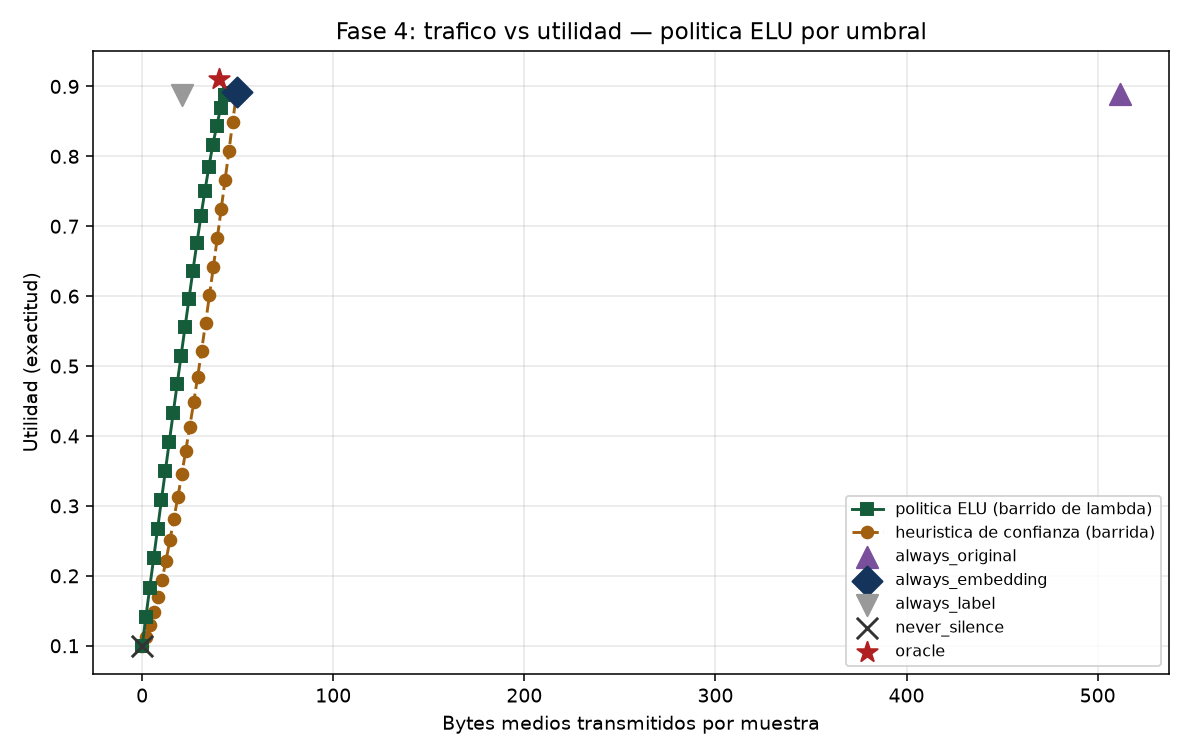
\includegraphics[width=0.82\linewidth]{results/figures/phase4_traffic_utility.png}
\caption{Fase 4: bytes medios vs. utilidad. La pol\'itica ELU domina a la heur\'istica de baja confianza en la curva evaluada y se aproxima al or\'aculo.}
\end{figure}

\textbf{Resultados.} El mejor punto ELU dentro de $\eps$ obtiene utilidad 0{,}8696 con 41{,}1 bytes medios, transmitiendo 83{,}3\% de las muestras. Frente a transmitir siempre la imagen original, reduce bytes en 92{,}0\% con p\'erdida menor a 3 puntos. Frente a transmitir siempre el \emph{embedding}, el ahorro marginal es 16{,}8\%. El or\'aculo alcanza un ahorro marginal de 19{,}1\% respecto a siempre-\emph{embedding}; por tanto, la pol\'itica ELU captura aproximadamente el 88\% de ese ahorro marginal no desplegable.

La comparaci\'on con confianza muestra que valor marginal e incertidumbre no son equivalentes. A fracci\'on transmitida igualada ($q=0{,}500$), ELU obtiene 0{,}5963 de utilidad frente a 0{,}4134 de la heur\'istica de baja confianza. En la curva evaluada, ELU domina a confianza. Este resultado depende del score usado, del respaldo por clase mayoritaria y de la calibraci\'on no expl\'icita del softmax; por ello se reporta como evidencia emp\'irica, no como garant\'ia universal.

% ==========================================================
\section{Criterios operativos de \'exito y falsaci\'on}

Los criterios operativos definidos para el proyecto acotado se cumplieron en estas corridas. La Tabla 5 resume la evidencia. Estos criterios no sustituyen una evaluaci\'on externa: delimitan qu\'e se considerar\'ia evidencia favorable o desfavorable dentro de este laboratorio.

\begin{table}[t]
\centering\small
\caption{Criterios operativos del proyecto acotado, evaluados en las corridas reportadas.}
\begin{tabular}{@{}p{0.56\linewidth}p{0.31\linewidth}c@{}}
\toprule
Criterio & Evidencia & Estado\\
\midrule
Una representaci\'on reduce $\ge$80\% los bytes con p\'erdida $\le$3 puntos & \emph{Embedding}: 90{,}2\%--97{,}4\% de ahorro (F1--F3) & $\checkmark$\\
Una representaci\'on aprendida supera a la compresi\'on cl\'asica en utilidad por byte, conservando utilidad & $\sim$7{,}9$\times$ (F2) y $\sim$19{,}1$\times$ (F3) frente al mejor cl\'asico dentro de $\eps$ & $\checkmark$\\
La pol\'itica por umbral reduce $\ge$50\% los bytes con p\'erdida controlada & 92{,}0\% frente a transmitir todo (F4) & $\checkmark$\\
El patr\'on de saturaci\'on utilidad--bytes es estable a trav\'es de semillas en las corridas principales & Las desviaciones observadas son del orden de $10^{-3}$--$10^{-2}$ y menores que las diferencias principales reportadas & $\checkmark$\\
\bottomrule
\end{tabular}
\end{table}

Los desenlaces de falsaci\'on estaban definidos: que el \emph{embedding} no conservara utilidad, que un cl\'asico dominara al \emph{embedding}, que el codo desapareciera en CIFAR-10, o que la pol\'itica por umbral no superara una heur\'istica simple. En estas corridas no ocurrieron. El resultado negativo m\'as informativo fue la ausencia de SSP visual: reducir la imagen de forma directa no conserv\'o la decisi\'on con ahorro suficiente.

% ==========================================================
\section{Reproducibilidad y artefactos}

El c\'odigo, las tablas, los reportes y las figuras se encuentran disponibles en el repositorio p\'ublico:

\begin{center}
\url{https://github.com/topassky3/tasknet-elu}
\end{center}

El DOI de Zenodo queda pendiente de publicaci\'on.

\textbf{Estado actual de disponibilidad.} Los resultados reportados provienen de los CSV generados por los scripts indicados en cada fase. El repositorio incluye las tablas, las figuras, los reportes de fase y los scripts principales de reproducci\'on.

\textbf{Artefactos disponibles.} El repositorio incluye scripts ejecutables y autocontenidos por fase, tablas CSV, figuras generadas por los scripts, informes y cierres de fase en Markdown, y un archivo \path{requirements.txt} con dependencias. Los scripts relevantes son \path{01_utility_per_bit_fashion_mnist.py}, \path{02_learned_vs_classic.py}, \path{03_cifar10_validation_v3.py} y \path{04_elu_threshold_policy.py}.

